\chapter{Introduction}

%\section{Bayesian Inference in modern science} % troppo lavoro e a me qui basta riassumere i passaggi

%inferenza bayesiana (figura semplice prior -> likelihood -> posterior), emulatori non cosmologici tipo speculator, emulatori cosmologici tipo cosmopower, ma sono tutti statici

%TEST CITAZIONE: \cite{cosmopower} \cite{precision_ml} \cite{islp} \cite{likelihood_cmb} \cite{understanding_ml} \cite{modern_cosmology}

% \section{Bayesian Inference Recap}
% \subsection{Bayesian Parameter Inference in Cosmology}

% \section{Bayesian Parameter Inference in Cosmology} % ancora non si parla molto di cosmologia qua...
\section{Bayesian Parameter Inference}
\subsection{Bayesian Parameter Inference: Conceptual Recap}
Bayesian methods have become a staple of modern science - and rightfully so, as they make the process of learning from data intuitive and rigorous; thanks to Bayes' theorem with only probability theory one can tackle common problems - such as parameter inference or model comparison - using a general, well-grounded approach. A Bayesian analysis is usually easier to interpret compared to its frequentist counterpart: the concept of probabilities as degrees of certainty about statements about the world is quite intuitive, and offers many other advantages - e.g. it removes the need to study the outcomes of other imaginary experiments one could have done. The main disadvantage of the Bayesian approach - i.e. the need for expensive computations - has stopped being an insurmountable obstacle in the era of cheap and powerful computers; still the computational side of a Bayesian analysis can pose nontrivial challenges, especially since in the last few decades the dimensionality of parameter spaces over which relevant posterior are defined has increased exponentially.
In particular in the context of cosmology there are peculiar computational challenges in applying Bayes' theorem: due to the unique properties of the problem at hand special tools have been developed to accelerate expensive analyses; in order to discuss these issues let us first recap the basic ingredients of a Bayesian analysis.

In the following we focus on the problem of parameter inference, i.e. trying to indirectly measure the value of some model parameters given a dataset about something else; even though the machinery of Bayesian statistics can also be applied to other problems (such as model selection) parameter inference is arguably both the simplest and most common scenario where one applies these tools. Parameter inference is usually the situation where students first familiarize themselves with Bayesian statistics, and is also especially relevant in cosmology, since inferring cosmological parameters from data about astrophysical objects is ``one of the cornerstones of modern observational cosmology'' \cite{cosmopower}. Finally we remark that the main topic of this thesis i.e. emulators in cosmology is about accelerating parameter inference pipelines - hence why we restrict our attention to this subset of what Bayesian statistics has to offer.

% \subsection{Inferring Parameters in Practice}
\subsection{Bayesian Parameter Inference: Practical Recap}
The starting point of the Bayesian approach to statistics is to treat model parameters as random variables and the available dataset as fixed. This reflects the idea that the dataset is just given to us, while with model parameters we use the ``notation of probabilities to represent [our] \emph{beliefs} about the mutually exclusive micro-hypotheses (here, values of [the parameters]), of which only one is actually true.'' \cite{mckay}. The idea is to use probabilities to denote degrees of belief given assumptions - hence why we use probability distributions to capture what we know about e.g. the value of a parameter.

All Bayesian pipelines hinge in some way on \emph{Bayes' theorem}:
\begin{equation*}
    P(\theta|D) = \frac{P(D|\theta) P(\theta)}{P(D)}
\end{equation*}
where we assume we have a dataset $D$ and model parameters $\theta$; each of the above probability distributions has a special name and meaning.

\paragraph{Prior distribution}
The distribution $P(\theta)$ is the \emph{prior Distribution}, and it represents prior beliefs, i.e. all the assumptions we enforce on the parameters $\theta$ \emph{before} seeing the data $D$. The prior can be used to express previous knowledge (for example it can be the posterior of a previous experiment) or assumptions (for example a reasonable prior describing a particle mass should be zero for negative values); otherwise one can use a ``blank'' prior, i.e. a distribution trying to express lack of previous knowledge about the parameters. Defining a good prior can be challenging; for example trying to make a prior uninformative in a parameter can result in a highly informative prior in a function of that same parameter (see for example \cite{noninformative_priors} \cite{nsb_prior}) - resulting in a biased posterior, requiring a switch of prior or the acquisition of more data.

\paragraph{Likelihood distribution}
The distribution $P(D|\theta)$ is called the \emph{likelihood distribution}; since this term is the protagonist of this work it deserves to have a unique symbol, hence in what follows the notation $\L(D|\theta)$ will be used. The likelihood is the part that captures the \emph{model} chosen to describe the physical process at hand; it is defined as the probability (density) of observing the dataset $D$ given that the model parameters are equal to $\theta$, but in a Bayesian context one usually ``flips it around''. What this means is that the expression of the likelihood is obtained as the probability of observing a dataset conditioned on known parameters, but then we fix the dataset equal to the obtained data samples and treat the likelihood as a function of the model parameters. Usually the likelihood contains both the physical model (a description of the part we actually care about) and the noise model (a description of the part we would like to remove but cannot), which requires one to have both relevant and nuisance parameters - the latter of which can be rigorously dealt with in a Bayesian setting thanks to marginalization.

\paragraph{Evidence}
The $P(D)$ term is called the \emph{evidence}. Even though in some problems its value plays a significant role (e.g. in model selection) in parameter inference it simply serves the purpose of regularizing the product of prior and likelihood, i.e. it ensures the resulting distribution's integral over all possible parameter values is 1. Indeed due to the rules of probability one can trivially check that the product of likelihood and prior is simply the joint probability distribution over $\theta$ and $D$, therefore its integral w.r.t. $\theta$ simply results in the marginal $P(D)$ - ensuring the ratio in the R.H.S. of Bayes' theorem is properly normalized. This marginalization makes it clear that the evidence represents the probability of observing the data irrespective of the value of the values of model parameters, i.e. this quantity is the union of all events leading to the dataset $D$ at hand - each with its own value of $\theta$.

Since the evidence is to be computed by integrating in parameter space over all possible $\theta$ value it becomes apparent that when the number of parameters is large (as has become more and more common over the last decades) this term can be basically impossible to compute; specialized techniques relying on \emph{Markov Chain Monte Carlo} methods have been developed to surmount the need to compute this quantity.

\paragraph{Posterior distribution}
The distribution $P(\theta|D)$ is called the \emph{posterior distribution}, and is the target of Bayesian inference. This distribution represents the updated beliefs about the parameters, \emph{after} learning from the data. The whole point of inference is to move from the prior to the posterior, i.e. to incorporate new knowledge about the world and let it modify previous beliefs. Superficially it seems as if the posterior distribution can be trivially obtained from Bayes' theorem once the prior and likelihood have been provided; in practice, though, this can be computationally expensive in all but the simplest of analyses. For example the evidence may be impossible to compute directly and indirect techniques may be needed, as described above; another common issue is that sometimes the likelihood is expensive to exactly evaluate, slowing down the whole pipeline process - hence why ``likelihood-free'' methods have found success in situations where the likelihood is expensive to evaluate but cheap to sample from (see \cite{astroabc} for a relevant cosmological example), which are common e.g. when the exact likelihood expression is known but requires an expensive normalization factor.

Once the posterior has been obtained it contains everything we could possibly want to know about the parameters; for example via marginalization we can obtain compact estimates for each parameter, we can compute credible regions, etc.

\subsubsection{Learning with Bayes' theorem}
The process of learning from data with a Bayesian parameter inference can be schematized as follows:
\begin{equation*}
    \text{Prior} \ P(\theta) \to \text{Likelihood} \ \L(D|\theta) \to \text{Posterior} \ P(\theta|D)
\end{equation*}
Paraphrasing the words of McKay \cite{mckay}:
\begin{quote}
    What you know about $\theta$ after the data arrive ($P(\theta|D)$) is what you knew before ($P(\theta)$), and what the data told you ($\L(D|\theta)$).
\end{quote}
The beautiful thing about Bayes' theorem is that it provides a way to intuitively and rigorously model mathematically the process of learning new knowledge about the state of the world, only relying on probability theory - therefore without the need to have a bunch of ad hoc tests and methods to come up with an answer about something.
Quoting \cite{doing_bayesian_data_analysis}:
\begin{quote}
    In summary, the essence of Bayesian inference is reallocation of credibility across possibilities. The distribution of credibility initially reflects prior knowledge about the possibilities, which can be quite vague. Then new data are observed, and the credibility is re-allocated. Possibilities that are consistent with the data garner more credibility, while possibilities that are not consistent with the data lose credibility. Bayesian analysis is the mathematics of re-allocating credibility in a logically coherent and precise way.
\end{quote}
% establish basic notation, scratch the surface...
Of course this discussion barely scratched the surface of what Bayes' theorem has to offer, both in theory and in practice. The point of this introduction is mostly to establish some basic notation and terminology that will be used extensively throughout the present work. The eager reader may find great resources about Bayesian analysis in \cite{mckay}, \cite{doing_bayesian_data_analysis}, \cite{jaynes_mysteries}, \cite{data_analysis_bayesian}, with \cite{trotta_sito} and \cite{trotta2017bayesian} being geared towards cosmology in particular.

\section{Emulators in Cosmology}
\subsection{Likelihood Emulation in Cosmology}
%descrivi a cosa servono e fai esempi di emulatori preesistenti
As described above in order to obtain a posterior one must be able to evaluate the appropriate likelihood - which can be computationally expensive. In particular in cosmology much work has been dedicated to the analysis of two-point statistics (power spectra or correlation functions); while this is appropriate (these observables carry a lot of information about cosmological parameters) it forces one to compute e.g. the theoretical power spectra corresponding to a given cosmological model i.e. a given set of values of the cosmological parameters. Indeed in inference pipelines of this kind the computational bottleneck is running exact Boltzmann solvers like \texttt{camb} \cite{camb} or \texttt{class} \cite{class_1} \cite{class_2}. A remarkable property of these spectra is that exact evaluations with repeated, expensive calls to these codes is often avoidable: \emph{in general cosmological power spectra are smooth functions of their input parameters} - hence why in the last 20 years many \emph{cosmological emulators} have been developed, i.e. fast and accurate surrogate functions that map cosmological parameters to the corresponding predicted power spectra.

\begin{equation*}
    \theta \mapsto P(\theta)
\end{equation*}
The idea is simple: since the above mapping between cosmological parameters and theoretical power spectra is usually regular, stable and smooth one can simulate a dataset of $(\theta, P(\theta))$ pairs (i.e. parameters values-corresponding spectra), then train an algorithm to learn this mapping as accurately as possible. It will then be possible to replace the expensive call to a Boltzmann solver with a quick one to the emulator: if training is successful the algorithm will both be able to reproduce spectra already presented to it (i.e. remember the dataset) and to accurately compute unseen before spectra, exploiting the smoothness of this mapping to fill the gaps in its knowledge of the $\theta \mapsto P(\theta)$ mapping (i.e. interpolate the dataset).
Thanks to emulation it becomes possible to have a once-and-for-all expensive training phase, after which power spectra can be obtained with a negligible loss in accuracy in the overall parameter inference with orders of magnitude speedups in the total computational overhead. 

The idea of accelerating inference pipelines with emulators has been successfully applied in many fields of science; this is especially true in the case of cosmology. The earliest successful attempts at emulation involved polynomial regression of power spectra \cite{emulator_poly_1} \cite{emulator_poly_2}; many emulators based on Gaussian Processes followed, applying these ideas to the emulation of matter power spectra \cite{emulator_gp_matter_1} \cite{emulator_gp_matter_2} \cite{emulator_gp_matter_3} \cite{emulator_gp_matter_4} \cite{emulator_gp_matter_5} \cite{emulator_gp_matter_6} \cite{emulator_gp_matter_7} \cite{emulator_gp_matter_8} \cite{emulator_gp_matter_9} \cite{emulator_gp_matter_10}, cosmic shear band powers \cite{emulator_gp_cosmic_shear_band_powers}, and Lyman-$\alpha$ forest flux power spectrum \cite{emulator_gp_lyman_1} \cite{emulator_gp_lyman_2}.
The recent surge in popularity of neural networks attracted the interest of the astrophysical community and ensured another batch of cosmological emulators relied on them - for the emulation of power spectra \cite{emulator_nn_matter_1} \cite{emulator_nn_matter_2} \cite{emulator_nn_matter_3} \cite{emulator_nn_matter_4} \cite{emulator_nn_matter_5} \cite{emulator_nn_matter_6}, angular power spectra of LSS observables \cite{emulator_nn_angular_lss}, global 21-cm signal \cite{emulator_nn_21_cm_1} \cite{emulator_nn_21_cm_2} \cite{emulator_nn_21_cm_3}, and to accelerate parts of Boltzmann codes \cite{emulator_nn_boltzmann}.
This list is clearly incomplete, as the literature is filled with several approaches to emulation; the important point to note is that emulation offers a practical and effective approach to significantly accelerate inference pipelines without significantly giving up accuracy.

One of the most recent emulation software packages is called \emph{CosmoPower} \cite{cosmopower}, which is ``a suite of neural cosmological power spectrum emulators covering both CMB (temperature, polarisation and lensing) and (linear and nonlinear) matter power spectra'' \cite{cosmopower}. Since its release CosmoPower has been further refined \cite{cosmopower_jax} and successfully applied in several contexts \cite{cosmopower} \cite{cosmopower_extra}; we remark that CosmoPower is especially interesting because it has all the best features of a modern cosmological emulator - hence why it was the main inspiration for the present work. Another important point is that most papers on emulators follow the same main steps outlined in \cite{cosmopower}, therefore by reviewing it we can gain insight on how emulators are designed and utilized in cosmology.

For all these reasons CosmoPower provides us with an excellent case study of what current cosmological emulators offer and how their potential shortcomings may be addressed using the approach outlined in the following chapters; therefore it pays off to recap the main results obtained in \cite{cosmopower}.

\subsection{\textit{CosmoPower}: a Case Study}
% figure dal paper, riassunto di come funzioni, cosa faccia, che risultati si ottengano, tutto molto sintetico
% ha senso
As previously mentioned CosmoPower is a collection of neural networks whose purpose is to emulate a set of relevant cosmological power spectra. Designing and implementing such networks requires a three-step process:
\begin{enumerate}
    \item Create a dataset by simulating power spectra for a range of cosmological parameters using exact Boltzmann solvers;
    \item Train the machine learning algorithm of choice after having optimized the relevant hyperparameters (see fig. \ref{fig:cosmopower_reti});
    \item Run statistical tests to ensure the accuracy of the networks' predictions; this is usually achieved by running the same inference twice (once with the ``true'' likelihood, once with the emulated one) and the comparing the posteriors.
\end{enumerate}
CosmoPower's predictor of choice is the simple feedforward fully-connected neural network regressor - whose activation functions, layer shapes, etc. have been chosen using a standard hyperparameter optimization approach.
\begin{figure}%[h]
    \centering
    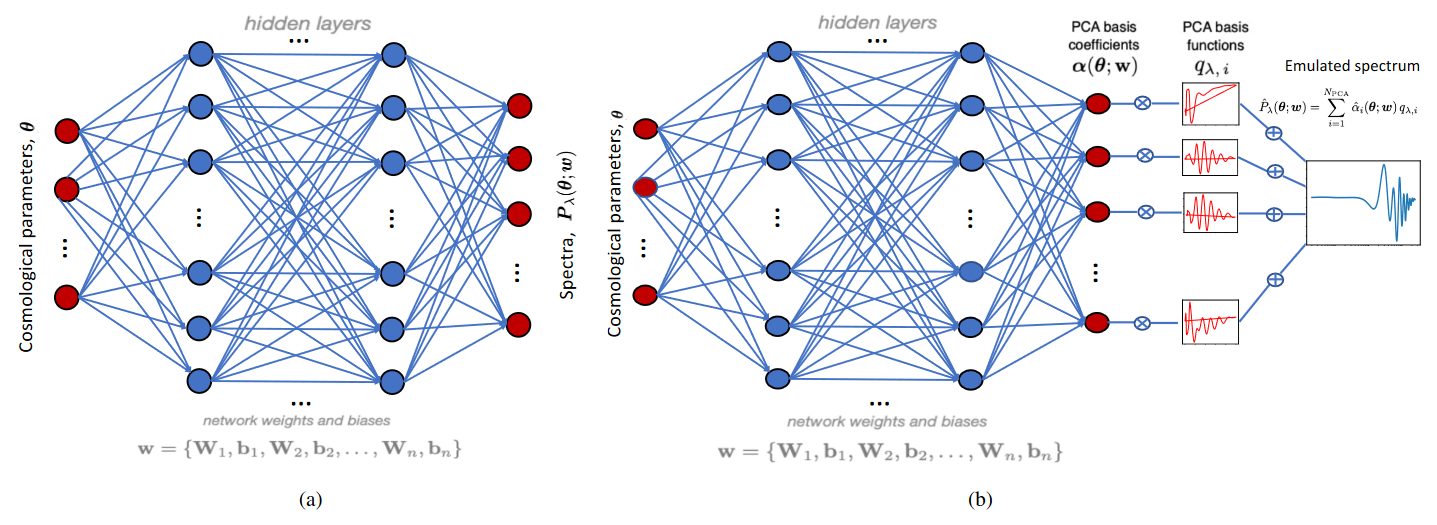
\includegraphics[width=1.0\textwidth]{img/cosmopower_reti.png}
    \caption{Types of neural networks implemented by CosmoPower: for some spectra the mapping from parameters to power spectra is learned directly, while for others the learned mapping is from parameters to the representation of power spectra in the basis induced by PCA.}
    \label{fig:cosmopower_reti}
\end{figure}
The paper goes into detail about all the technical issues regarding the production of the datasets from the available codes as well as other factors that are beyond the scope of this work; the important result is that using these networks is possible to obtain accurate posteriors with impressive speedups - a good example of which is reported in fig. \ref{fig:cosmopower_contours}.
\begin{figure}[h]
    \centering
    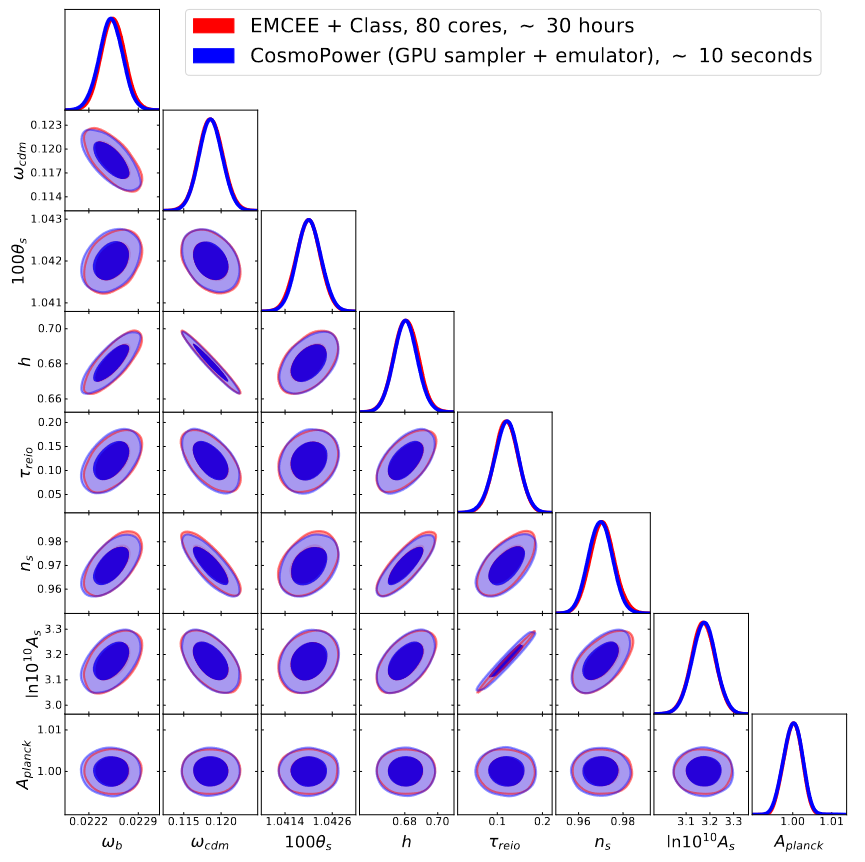
\includegraphics[width=1.0\textwidth]{img/cosmopower_contours.png}
    \caption{Comparison between exact codes and CosmoPower while performing a Planck 2018 3$\times$2pt analysis. We notice that the difference between posterior contours is quite small, whereas the difference in compute time is much more noticeable (in some of their analysis in \cite{cosmopower} the authors are able to replace an almost week-long computation with one lasting few hours).}
    \label{fig:cosmopower_contours}
\end{figure}
The main point is that one can obtain great emulators in a relatively simple way. In particular CosmoPower is a fast, accurate, differential, flexible, GPU-compatible emulator, capable of interfacing with arbitrary cosmological samplers thanks to its ``train-once-use-repeatedly'' approach - while also offering extra features, like the ability to compute derived quantities without re-training.

% (in this case a few simple feedforward fully-connected neural network regressors) (activation function, network shape, etc.)


\subsection{\textit{CosmoLIME}: A new kind of Cosmological Emulator}
\begin{comment}
riassunto di cosa fanno tutti: 1) genera il dataset 2) addestra il modello 3) confronta l'esito di una inferenza con quello fatto con la likelihood esatta = approccio statico (riconnettiti a quanto descritto sopra per cosmopower)
->
ripartire completamente da zero: scambiare modelli con stessi dati, cambiare dati
tradeoff fra computer time e human time: quando tutto è finito risparmio tempo nella inference (poco computer time ignorando il training, che comunque è una tantum e poi mi permette di fare tutte le analisi del mondo) ma prima devo fare tante prove io di modelli, ottimizzazione, decidere prima il dataset, eccetera


le features che vorremmo:
- likelihood arbitraria
- modelli arbitrari
- preprocessing arbitrario
- tutto automatico: target, scores, eccetera
- test statistici?
- features carine: caching, logging, parallelizzazione, vedi agende varie su keep

molto importante: le caratteristiche uniche del problema (se non qui da qualche altra parte). Cioè: likelihood in generale regolari -> è possibile una emulazione efficace, dati simulati -> non siamo limitati ad un dataset prefissato.
Dati infiniti e senza errori vari = possiamo spingerci a loss bassissime tipo precision machine learning (cita paper)

Nota su quanto sopra: negli esempi di osservabili del prof quanto sopra è sicuramente vero (dati 100\% simulati), ma che mi dici ad es di cosmopower o simili? (anche solo l'esempio dell'energia oscura)

Questi casi sono ibridi; certamente servono dei dati da inserire ma questi spuntano nella forma ad es di matrici di covarianze di gaussiane - che una volta specificate ci fanno rientrare nello scenario di dati potenzialmente infiniti. (altro esempio i coefficienti C ell, che però essi stessi altro non sono che una rappresentazione alternativa di una likelihood la cui forma generale è nota a meno della parte in cui entrano i dati...? Verificare!)

Si può comunque specificare che cosmolime supporta anche i casi di dataset fissati, che possono essere visti come un sottoinsieme del caso più generale (cioè come ad esempio un'unica passata di sampling, un'unica generazione di dati)
\end{comment}
\subsubsection{The shortcomings of the out-of-the-box approach}
Emulators like CosmoPower can be of great help to the astrophysical community: a researcher eager to run inference pipelines on e.g. new data can accurately and quickly do so. And yet the ``train-once-use-repeatedly'' approach, which is the software's main strength, can also be its strongest weakness. Indeed while it is true that under the right conditions emulators like CosmoPower can be safely utilized out-of-the-box one can also easily imagine situations where these conditions do not apply.

\paragraph{Failure to meet accuracy requirements}
% pagina 12 da We note that a Stage IV surveys
The predictors inside CosmoPower obey the same rules as most supervised learning algorithms; in particular training continues until an appropriately defined test error is low enough - for example one can ensure the residuals between predicted and true values are small enough. But how can one choose how low is low enough? A value of the test error may superficially seem small while still leading to biased posterior estimates. The authors of CosmoPower themselves warn against training an emulator without checking its performance in a realistic inference pipeline; simply checking the residuals may fool one into believing the emulator is accurate enough for the inference at hand.
Quoting from \cite{cosmopower}:
\begin{quote}
    We note that applying the emulator to a complete inference analysis from a simulated Stage IV survey, as done in our paper, is a necessary step to ensure that the newly developed tool can be safely applied in practical analyses. On  the contrary, checking residuals in the testing set between predicted and real spectra is not a sufficient accuracy test. While an emulator may be performing with e.g. subpercent accuracy at the level of residuals, this may still not be enough to retrieve unbiased cosmological contours, as we verified first-hand while testing \textsc{CosmoPower}. This is due to the fact that the accuracy threshold for the emulation can only be defined by the specific application for which these emulators are designed. In other words, it is the inference pipeline that dictates the accuracy threshold to be met by the emulator. In general, parameter estimation in Bayesian inference pipelines requires a certain level of accuracy in the observables computed, which in the specific case of cosmological two-point statistics analyses reflects into certain accuracy requirements in the power spectra computed by Boltzmann codes. Hence, we argue that the principled approach to validate an emulator accuracy is to compare its performance within an inference pipeline for a target experiment, which in our case is a Stage IV survey configuration. Note that, while testing \textsc{CosmoPower}, we experienced first-hand that emulators performing greatly on Stage III experiments failed in producing equally correct contours on a simulated Stage IV survey.
\end{quote}
The accuracy of the emulator is critical to ensure it can safely replace exact codes; no one will give up significant accuracy with computational speedups. Imagine if a user is not sure a priori whether the available emulator is accurate enough for their purposes; according to the very authors of CosmoPower the wise choice is to perform a side-by-side comparison of exact and approximate inferences - but \emph{this defeats the very purpose of an emulator}, which is to be able to avoid costly exact computations. It's not impossible that one may be able to salvage something - for example testing the accuracy of the emulator once or on a subset of the dataset and then using it in other situations with the same conditions; but what about an even worse situation? In particular if a user is sure a priori that the already existing emulators simply are not accurate enough to be used for the task at hand then all the nice ``train-once-use-repeatedly'' approach simply fails and readily available emulators like CosmoPower cannot be employed.

To recap: if the authors of an emulator cannot guarantee the required accuracy of their software then using it ``as-is'' becomes either impossible or forces the user to prove themselves that the emulator is appropriate for the relevant task; in either case the out-of-the-box functionality is no longer present.

\paragraph{The need to change model or preprocessing}
When ``shopping'' for an emulator the user is forced to comply with the approach of the authors. Each of the available emulators is designed to achieve certain properties (e.g. the rigorous uncertainty propagation made easy by Gaussian Processes) and/or the best performance under some design constraint (e.g. picking the shape of a neural network according to some hyperparameter optimization technique), but what if the user wishes to try different choices? For example if another preprocessing transformation is deemed better using the available emulators becomes suboptimal; the same holds if other machine learning algorithms seem more appropriate - for example in \cite{cosmopower} the authors state their desire to try Bayesian neural networks to replicate the uncertainty propagation properties of Gaussian Processes, and also to try more interpretable machine learning algorithms. In general while the exact computation is ``unique''\footnote{Of course the reality of this issue is not so simple: different softwares may use different computational methods or physical models to reach the results. What we mean is that performing an exact computation does not require as many arbitrary design choices as picking a regressor/preprocessing transformation/etc..} the road to emulation is not; emulation relies on a series of design choices by the authors, choices one may disagree with or find suboptimal. %Even though this situation may simply seem the outcome of the pickyness of a user in particular it actually happens naturally: as new algorithms become popular new software is released, superseding outdated ones. The same happens when new theoretical codes are released: if it becomes possible to produce more accurate datasets

\paragraph{The need to emulate different likelihoods}
% altre situazioni o cosmologie o teorie o che ne so
% parameter range come dicono in flexibility in cosmopower, o altre cose tipo la derivabilità. Loro ce l'hanno ma altri no, a tipo
Designing an emulator is more than just picking a preprocessing transformer and a regressor: in order to produce the dataset used to train any emulator one must choose appropriate exact codes, which means choosing a particular cosmological model. Even within the same model there are choices to be made about the physics of the problem (which parametrization to use? Within which range are the parameters to be sampled?); finally once the emulator is trained it is also tested against a particular experimentally obtained dataset. Once again this may be limiting if the available and desired emulators do not line up; for example in the conclusions of \cite{cosmopower} the authors state their desire to extend CosmoPower to the prediction higher order statistics and/or to other cosmological models.


\subsubsection{The trade-off between human time and computer time}
% descrivere che tutte le situazioni viste sopra hanno in comune il bisogno di ricominciare da zero il training, quindi anche se nel lungo termine si risparmia computer time nel breve termine bisogna sacrificare un sacco di human time (certamente cercare un software su arxiv o github è più rapido di farselo da soli)
% allora sarebbe simpatico avere un framework standard che permetta di specificare relativamente poche informazioni e che premendo play permetta di rifare tutto daccapo senza pensarci troppo (lista delle desiderata)
All the situations outlined above share one common property: \emph{the failure of the out-of-the-box approach}. If the available emulators cannot guarantee the desired features (accuracy, statistical and physical properties, etc.) then the user cannot use them ``as-is''. The important thing to note is that these situations do not necessarily forbid the use of emulators - just that of the already available ones. What we face is therefore \emph{a trade-off between human and computer time}: on one hand in the long run an emulator can save \emph{computer time} (after training\footnote{Of course if an emulator is trained from scratch at least some computer time is needed to simulate the dataset, run the training algorithm, then perform the side-by-side test inferences. The out-of-the-box approach relies on the idea that this time can be spent once, so that no one else has to; but even if the user themselves has to spend this time an emulator can still be useful, at least as long as the future inferences are much more costly than the training of the emulator itself.} inferences take a fraction of the time), but on the other in order to successfully implement an emulator \emph{from scratch} a lot of \emph{human time} may be needed - to choose between different models, etc.

\subsubsection{Introducing CosmoLIME: from prebuilt to DIY emulators}
% standardized, plug-and-play approach
Having outlined how and why the need for retraining cosmological emulators may arise we ask what can be done about it; we argue that a change of approach may be fruitful. In particular we ask: what if instead of trying to implement a bunch of emulators (each with its own ``area of expertise'') we wrote a software that allowed everyone to assemble their own emulator? As said above training a tailored emulator may be unavoidable, and this requires a sacrifice of human time; our idea is to minimize this time by streamlining the process needed to obtain a functional emulator.

We know that building an emulator is a three-step process:
\begin{enumerate}
    \item Generate a dataset via simulation;
    \item Train a (set of) machine learning predictor(s);
    \item Test the result with metrics based on realistic inference pipelines.
\end{enumerate}
Since these steps are always the same we argue that it should be possible to create a framework in which these steps take a standardized, plug-and-play form. If such a framework could be built the user would simply need to specify how the dataset should be generated (i.e. the physics of the problem) and which preprocessing transformer/regressor to use; then it would be simply a matter of ``pressing play'' and let the software handle the optimization and testing of the user-proposed algorithms. A software framework like this could allow the user to once again have an emulator already made for them by someone else - except that in this case there would be no need to accept the design choices imposed by others, since the resulting emulator would be tailor made for them.

What we propose here is therefore a \emph{change of paradigm}: we propose moving away from ``statically-generated'' emulators (i.e. built once by others, then set in stone), switching to the new ``dynamically-generated'' kind. From the point of view of the user nothing has changed, as in both case the user ``orders'' an emulator; what changes is that instead of picking from a fixed menu the user can now request arbitrary dishes, tailored to their taste and needs. 
Let us then specify all the desired properties of this new idea of a software emulator; such a ``wish-list'' can then be used to define guidelines useful in designing this new software.

\begin{comment}
% FINIRE QUA
\paragraph{Custom made emulators}
% non voglio dare un emulatore pronto ma piuttosto gli ingredienti per costruirlo da sé. è la differenza fra comprare un prodotto già fatto e uno a pezzi tipo i lego o ikea: te lo fai da solo ma in modo guidato.
As said above this new approach to emulation consists of automated DIY. This can be achieved by building a software that accepts as input a list of parameters expressing all needed parts (the model to be optimized, the rules for generating the dataset, etc.), then assembles them on its own.

\paragraph{Support for arbitrary likelihoods}
% sia nel senso che vorrei poter cambiare problema sia nel senso che nel contesto dello stesso problema vorrei poter cambiare modello cosmologico, parametrizzazione, range entro cui vengono campionati i parametri durante la generazione, eccetera
Each of the already available emulators focuses on a specific likelihood, with a fixed set of physical assumptions; within our framework it should be possible to change them. In particular current emulators rely on a specific

\paragraph{Support for automated data generation}
% discorso dei dati simulati, eccetera

\paragraph{Support for arbitrary ML models}
% non devi essere un esperto e decidere a priori il modello, magari gliene dai tanti e se la sbriga lui

\paragraph{Support for arbitrary preprocessing}
% anche una default option ci piace

\paragraph{Support for automated testing}
% le inferenze non si possono generalizzare più di tanto, ma puoi fare i test di ML soliti (test eccetera), loss che  tengano d'occhio le robe in corso d'opera (tipo il chi^2 del prof), e forse creare una interfaccia con dei samplers o robe del genere? Mi sa di no

\paragraph{Other useful features}
% caching eccetera
\end{comment}

\paragraph{Dynamic emulation framework features wish-list}
\begin{itemize}
    \item Custom made emulators: we aim for an automated DIY approach to emulation, as explained above.
    \item Support for arbitrary likelihoods: we aim to support the emulation of any function in order to support the broadest range possible of physical problems - for example the emulation of different power spectra, or the same spectra but under different cosmological models, or the same model but with different parametrizations or parameters sampled in different ranges, etc..
    \item Support for automated data generation: since the datasets relevant to emulation are obtainable via simulation there are no hard limits to the number and quality of the generated samples (i.e. no fixed number of available data, no experimental errors, etc.); therefore instead of dealing with an a priori fixed dataset it makes sense to define a framework in which data samples are generated automatically when needed.
    \item Support for arbitrary ML models: to ensure maximum user freedom we wish to have an algorithm where the machine learning predictor employed is arbitrary; this can be achieved by having the model be just a variable argument used as input to an empty slot in an otherwise unchanged standardized procedure.
    \item Support for arbitrary preprocessing: similar to the previous point, with the added point that it makes sense to provide reasonable default options.
    \item Support for automated testing: the final accuracy test of an emulator is the side-by-side inference, as explained above; this requires external elements (i.e. an experimentally obtained dataset and a posterior-sampling algorithm) that are probably best left in the hands of the user. Still it can be useful to have some default options to automatically perform a test inference, requiring only the external dataset; on the other other statistical tests can still be automatically performed by the framework, such as the computation of the test error, $\chi^2$ or other useful quantities.
    \item Other useful features: several other technical features should be included in a software framework like this. Examples include support for caching (saving of intermediate results), logging (output of current algorithm state), parallelization (both in the data generation phase and to test multiple models concurrently), etc.
\end{itemize}


\paragraph{CosmoLIME}
% We present \textsc{CosmoLIME}, the \textit{Cosmological Likelihood Machine learning Emulator}. \textsc{CosmoLIME} is \emph{the} cosmological emulator (instead of \emph{a} cosmological emulator) because instead of being an emulator in particular it is \emph{all of them}, in the sense that it is a software framework designed and implemented according to the above guidelines. As such it allows the user to generate custom-made emulators with a seamless, standardized approach satisfying all the desirable features described above. As such \textsc{CosmoLIME} is a ``universal'' emulator; it is so general that it can actually be used in arbitrary machine learning problems - as long as the data can be simulated instead of being fixed, that is.
We present \textsc{CosmoLIME}, the \textit{Cosmological Likelihood Machine learning Emulator}. \textsc{CosmoLIME} is not an emulator in the sense that it provides the user a ready-made likelihood replacement for a specific problem under a certain set of assumptions; it instead is a software framework designed and implemented according to the above guidelines. As such it allows the user to generate custom-made emulators with a seamless, standardized approach satisfying all the desirable features described above. This ensures \textsc{CosmoLIME} is a ``universal'' emulator; it is so general that it can actually be used in arbitrary machine learning problems - as long as the data can be simulated instead of being fixed, that is.

The remainder of the present work will describe how \textsc{CosmoLIME} works, discuss some simple applications and propose possible enhancements to be implemented in the future.